\documentclass[12pt]{article}
\setlength{\textheight}{210mm}
\addtolength{\topmargin}{-18mm}
\setlength{\textwidth}{165mm}
\setlength{\oddsidemargin}{5mm}
\usepackage[labelfont=bf]{caption}
\usepackage{graphicx, subcaption, amsfonts, amsmath}
\usepackage{tikz}
\graphicspath{ {./figs/} }
\pagestyle{plain}
\begin{document}
\title{Manifold Learning to Enable Equation-Free Modeling of Chemical Engineering Systems}
\author{\LARGE Proposed by David Sroczynski\vspace{3mm}\\\Large under the supervision of\vspace{3mm}\\\LARGE Professor Yannis Kevrekidis}
\date{12/04/2015}
\maketitle
\thispagestyle{empty}
\clearpage
\tableofcontents
\thispagestyle{empty}
\clearpage
\pagenumbering{arabic}
\section{Introduction}
Many fields of science and engineering use modeling to expand and elucidate the information available from experiments. These models range from simple, one-variable ODEs for a stirred-tank reactor to computational fluid dynamics code. Experimental data is generally noisy and incomplete; a well-developed model can bring clarity to complicated systems. Models have the additional advantage that they can be initialized as often as desired in whatever state is desired, while experiments can be challenging or expensive to initiate. The obvious caveats are that a model must be accurate enough to capture the ``important" information while being compact enough to be solved in a reasonable timeframe.  \vspace{1mm}

The field of dimensionality reduction explores the question of what information is ``important." The concept is very old; for example, we learned early on that in the analysis of a chemical reaction, the important variables often include concentrations and temperature, which are spatial averages of molecular counts and speeds. The reaction may involve collisions between individual molecules, but we only need to know the value of these average properties to predict the average behavior. In other words, the reduced set of variables constitutes a closed-form, self-contained system. As we attempt to model new or more complex systems, we desire more systematic ways to extract these important variables from the available data. The most ubiquitous method is principal component analysis (PCA), which can be traced back to as early as 1901 \cite{Pearson1901}, but was developed across many fields under many names over much of the $20^{th}$ century \cite{Hotelling1933, Sirovich1987}. PCA can be thought of as an extension of the line-of-best-fit method to higher dimensions: if the data is viewed as a cloud of points in some high dimensional space, PCA determines which directions characterize the highest variability in the data. Projecting the data onto only these directions results in a reduced representation of the data that still captures most of the variability. One drawback to PCA is that it only captures linear relationships (consider the case of a line-of-best-fit vs. a nonlinear curve fit). The field of nonlinear dimensionality reduction has grown rapidly in recent years with the introduction of methods like kernel PCA \cite{Scholkopf1998}, local linear embedding \cite{Roweis2000}, Isomap \cite{Tenenbaum2000}, Laplacian eigenmaps \cite{Belkin2003}, and diffusion maps \cite{Coifman2005, Coifman2005a, Coifman2006}. By capturing nonlinear structure, these methods can reduce data further than linear methods while maintaining a similar amount of important information. \vspace{1mm}

Dimensionality reduction methods have the potential to greatly improve clarity and speed of models by reducing the model to lower-dimensional representations that are easier to visualize and faster to compute. We are interested in using diffusion maps to improve model efficiency in molecular simulation and other relevant chemical engineering systems. Diffusion maps has recently shown promise in data analysis for models in transport \cite{Sonday2009}, chemical kinetics \cite{Chiavazzo2014}, and molecular dynamics \cite{Ferguson2010, Ferguson2011, Nedialkova2014, Kim2015}. We intend to expand on this work in the context of the ``equation-free" (EF) framework \cite{Kevrekidis2004}, which uses short simulations of detailed models as the basis for projection in a reduced model. EF is useful when good reduced variables are known but do not have closed-form equations; diffusion maps can be used to find the reduced variables. This idea of data analysis for the purpose of computation includes the idea of aiding in the development of a model or the characterization of dynamical systems by biasing where to next initialize simulations to gain ``important" information. This in particular has applications to molecular simulation, where the characterization of rare events can be extremely expensive; methods to speed up these computations often require a good reduced variable to bias the simulation.  \vspace{1mm}

This document will first explain the EF framework and then discuss diffusion maps and some of the challenges in its implementation. We will describe current work being done on a data-centric application in developmental dynamics, and then we will conclude with systems of interest in future work.  \vspace{1mm}

\section{Equation-Free Modeling}

EF modeling refers to the framework of using exisiting detailed microscopic simulators in a black-box manner to enable solutions to macroscopic tasks that are intractable for the microscopic simulator in its original formulation \cite{Siettos2003, Kevrekidis2003, Kevrekidis2004}. Consider such a simulator (e.g., molecular dynamics or computational fluid dynamics code) which performs detailed simulation (i.e, time-stepping on the microscopic level) given certain initial conditions and parameters. EF modeling requires the existence of an appropriate coarse (low-dimensional) description, where appropriate in this context means that it should capture the ``important" information. We want the detailed simulation to evolve along some lower dimensional manifold (which can be parameterized by our coarse variables) embedded in the detailed, high-dimensional space. Simulations that are initialized away from this manifold should very quickly move to the manifold in the spirit of chemical kinetics systems where some species can be assumed to follow the quasi-steady-state approximation, which constitutes an effective dimensionality reduction. \vspace{1mm}

EF modeling also requires two operators for moving between coarse (low-dimensional) and fine (high-dimensional) descriptions. A restriction operator converts a fine description to a coarse description; for example, the coarse variable temperature can be considered as a restriction of the speeds of each molecule in MD simulation. Lifting operators, which do the reverse, often have the added complication that there are many fine descriptions that correspond to the same coarse description, so some care needs to be taken in systematically choosing a fine description. In many cases, however, even if the fine simulation is initialized poorly, it will quickly move back to the appropriate manifold. This quick relaxation is typically referred to as healing. \vspace{1mm}

Given the detailed simulator, the appropriate coarse description, and the two operators, the most straightforward application of the EF framework is coarse projective integration (CPI), where we step the coarse variables forward in time based on fine simulations initialized according to the lifting operator. For each coarse integration step, the procedure is as follows (see Figure~\ref{fig:cpi} for a schematic):  \vspace{1mm}

\begin{enumerate}
\item Use the lifting operator to determine initial conditions for the fine simulation based on the current values of the coarse variables.
\item Run the fine simulation for a short healing period to bring it back to the appropriate manifold.
\item Continue to run the fine simulation long enough to determine the rate of change of the coarse variables.
\item Project the coarse variables forward in time using forward Euler integration or any other integration scheme.
\end{enumerate}

If the simulation data actually lie on or near a manifold characterized by the coarse variables, coarse projective integration offers vast speed-ups compared to straight integration of the fine simulation. This framework of using fine simulations to determine the coarse behavior also has applications in stability/bifurcation analysis \cite{Theodoropoulos2000, Gear2002} and the exploration of potential surfaces \cite{Frewen2009}. We are interested in applying this approach to systems where the coarse variables are not known \textit{a priori} but must be determined through dimensionality reduction. \vspace{1mm}

\tikzstyle{block} = [rectangle, draw, fill=blue!20, 
    text width=5em, text centered, rounded corners, minimum height=4em]
\tikzstyle{line} = [draw, -latex]
\begin{figure}[here]
\begin{tikzpicture}[node distance = 2cm, auto]
	\node [block]  (Cinit) {Coarse description at time $t$};
	\node [block, below of=Cinit, node distance=3cm] (Finit) {Fine description at time $t$};
	\node [block, right of=Finit, node distance=7cm] (Ffinal) {Fine description at time $t+\delta t$};
	\node [block, above of=Ffinal, node distance=3cm] (Cfinal) {Coarse description at time $t+\delta t$};
	\node [block, right of=Cfinal, node distance=7cm] (Cproj) {Coarse description at time $t+\delta t + \Delta t$};
	\path [line] (Cinit) -- node {Lifting} (Finit);
	\path [line] (Finit) -- node {Detailed simulation} (Ffinal);
	\path [line] (Ffinal) -- node {Restriction} (Cfinal);
	\path [line] (Cfinal) -- node {Numerical integration} (Cproj);
\end{tikzpicture}
\caption{\textbf{Schematic for a coarse projective integration step.} There is significant speedup if $\Delta t$ can be chosen much larger than $\delta t$ while maintaining reasonable accuracy.}
\label{fig:cpi}
\end{figure}

\section{Diffusion Maps}

\subsection{Overview} \label{DMO}

Diffusion maps is a method of analyzing the geometry of data and discovering lower-dimensional manifolds that the data approximates (for an example, see Figure~\ref{fig:sr}). The algorithm is designed to approximate the eigenfunctions of the continuous Laplace-Beltrami operator (which have been shown to provide good parametrizations of nonlinear manifolds \cite{Jones2008}) to discrete data. Suppose you have \textit{m} data points in \textit{n}-dimensional space represented by $y_1$,...,$y_\textit{m}$. The algorithm first constructs a weight matrix such that $\exp$\\
\[
W_{ij}=\exp{\left(-\frac{||y_i-y_j||^2}{\sigma ^2}\right)}
\]
where $|| \bullet ||$ is an appropriate norm or distance metric between two data points and $\sigma$ is a characteristic distance such that points are considered similar. Diffusion maps treats distances smaller than $\sigma$ as important but treats distances much longer than $\sigma$ as meaningless. The matrix is then made row-stochastic by dividing each row by its sum so that the rows sum to $1$. This gives $W$ the interpretation of a Markov matrix such that the elements represent transition probabilities from one data point to another, thereby modeling random walk diffusion among the data points. Variations to the algorithm exist which can, among other things, account for variations in sampling density \cite{Coifman2006}.\vspace{1mm}

The eigendecomposition of W yields eigenvalues $\lambda _0$,...,$\lambda_{m-1}$ and eigenvectors $\phi _0$,...,$\phi_{m-1}$. Due to row-stochasticity, the first eigenvector $\phi_0$ is a trivial constant vector with $\lambda_0 = 1$. The other eigenvectors provide a new coordinate system such that the $k^{th}$ component of $y_i$ is given by the $i^{th}$ component of $\phi_k$, scaled by $\lambda_k$. It has been shown that in this new coordinate system, Euclidean distance between two points approximates a quantity referred to as the diffusion distance \cite{Coifman2006}. This diffusion distance represents moving from one point to another by random walk diffusion, where you can only move to nearby points based on the probabilities in the weight matrix. Since diffusion distance is based on moving from point to point, it approximates the distance along the manifold that the points lie on. If there is a large spectral gap, meaning that some eigenvalues are significantly larger than others, then the diffusion distance can be accurately approximated using only coordinates with the largest eigenvalues.  The number of these large eigenvalues gives information about the true dimensionality of the manifold. One complication is that since the true eigenfunctions of the Laplace-Beltrami operator (the diffusion operator which we have approximated) are periodic, not all coordinates will parameterize new directions on the manifold, but will instead be higher harmonics. Methods have recently been proposed to automatically identify and remove these coordinates, which allows for maximum dimensionality reduction \cite{Dsilva2015}.

\begin{figure}[here]
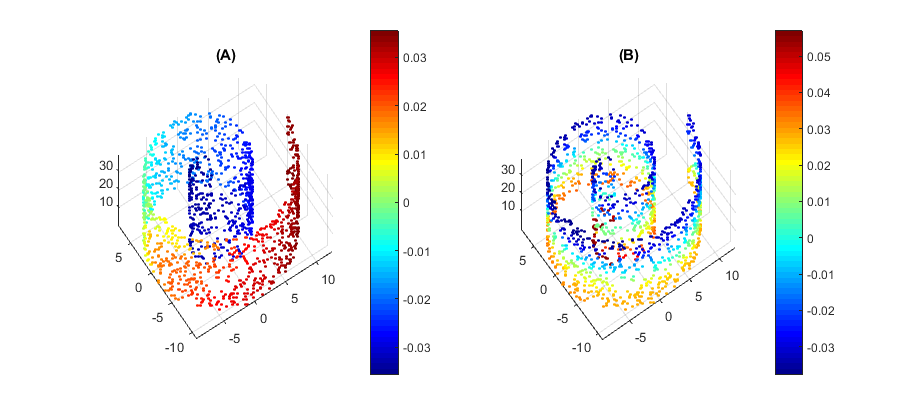
\includegraphics[width=\linewidth]{figures/swissroll}
\caption{\textbf{The canonical manifold learning example: the Swiss roll}. 1500 points randomly sampled from a Swiss roll, colored by the (A) first and (B) second diffusion maps coordinates. The first coordinate paramterizes arc length along the swiss roll, while the second parameterizes the height. Although the original data is in three dimensions, it can be more simply described by just those two.}
\label{fig:sr}
\end{figure}

\subsection{Choosing a distance metric and kernel scale}

Since the diffusion maps algorithm is based entirely on the distances between points, choosing an approriate distance metric is critical. Assuming that each data point is represented by a vector such that each element represents one variable that describes the state (e.g., concentration of one chemical species, signal intensity at some point in space, etc.), then the obvious solution is simply the Euclidean distance between the two points described by the two data vectors. Unfortunately, in many instances, straightforward application of the Euclidean distance is not an informative measure of similarity. Here is a listing of some useful modifications and alternate approaches:

\begin{enumerate}
\item \textbf{Data preprocessing.}  This is a general term for adjusting the data, either manually or systematically, so that the Euclidean distance becomes more informative. This can include actions like standardization of variables which span disparate scales, blurring of spatially organized data to remove uninformative small-scale structure, and contrast boosting or other image enhancement.
\item \textbf{Feature extraction.} In certain cases, \textit{a priori} knowledge about the system can justify the selection of informative features. These functions of the original data can include ratios of quantities, times to achieve certain benchmarks, or quantities of distributions. For example, in a particular molecular simulation, it may already have been shown that important features include average kinetic energy per particle or the peaks in the radial distribution function. This is essentially an initial step of dimensionality reduction before allowing the formal algorithm to finish the job. Unfortunately, this \textit{a priori} knowledge is often unavailable for new systems.
\item \textbf{Mahalanobis distance }\cite{Dsilva2015, Dsilva, Mahalanobis1936}\textbf{.}  This metric is primarily useful in stochastic systems where movement along the slow manifold is obscured by independent white noise. Based on the covariance of the data, the Mahalanobis distance ignores directions which do not indicate meaningful dissimilarity. Given column vector observations $y_i$ and $y_j$ from a distribution with covariance $C$, the Mahalanobis distance is given by
\[
||y_i-y_j||^2_M = (y_i-y_j)^TC^{-1}(y_i-y_j)
\]
The covariance matrix typically must be estimated from the data, and often the estimation is not full-rank so a pseudoinverse is required. For an example of where this is useful, see Figure~\ref{fig:mahalanobis}.
\item \textbf{Earth mover's distance }\cite{Levina2001}\textbf{.}   Initial feature extraction sometimes motivates the use of distributions on each data point rather than the raw data (e.g., when each data point describes a collection of interchangeable particles). Also known as the $1^{st}$ Wasserstein metric, the earth mover's distance quantifies how much work is required to change one histogram into another; in the limit of infinite data and discretization, EMD compares probability distributions.
\item \textbf{Graph metrics.} A graph is a representation of data that defines nodes (which can be people, websites, locations, etc.) and edges (connections) between nodes. These edges can be either weighted or unweighted, and either directed or undirected. Methods for graph similarity include edit distance, maximal common subgraph, and graph kernels. These methods are often computationally intractable, but methods exist for their approximation.
\end{enumerate}

Once the distance metric is chosen, the kernal scale $\sigma$ must also be chosen. This sometimes requires trial and error, but a good initial guess is to use some fraction (e.g., $\frac{1}{2}$) of the median pairwise distance between data points. An alternate approach is to use the maximum distance to some number of nearest neighbors, averaged over each data point.

\begin{figure}[here]
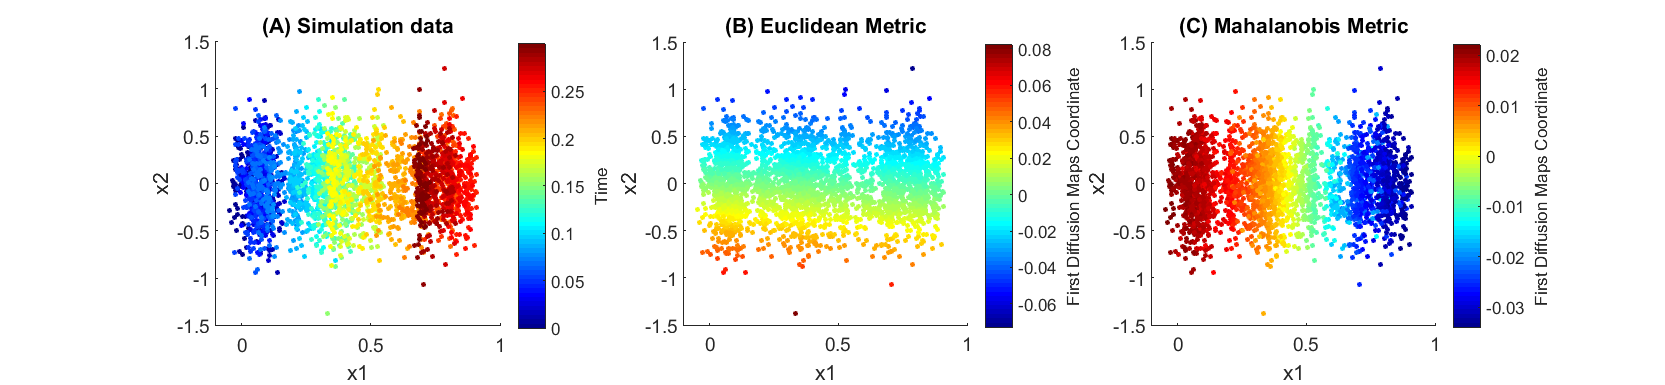
\includegraphics[width=\linewidth, clip=true, trim=115 0 75  0]{figures/my_mahalanobis}
\caption{\textbf{Benefits of the Mahalanobis distance.} (A) Results of a stochastic simulation colored by time. The slow variable ($x_1$) gradually drifts from left to right over the course of the simulation. The dynamics are obscured by a fast variable ($x_2$) which has mean $0$ but large Brownian motion. (A) Data points are colored by the first diffusion maps coordinate using the Euclidean distance. We recover the fast variable, which gives no information about the state of the system. (B) Data points are colored by the first diffusion maps coordinate using the Mahalanobis distance. We recover the slow variable, which is much more indicative of the state of the system. More analysis can be found in \cite{Dsilva2015}.}
\label{fig:mahalanobis}
\end{figure}

\subsection{Synchronization of data: factoring out symmetry}

Another issue that can occur in the application of diffusion maps is when data points have some degree of freedom among some symmetry group that obscures the dynamics. We would like to factor out the effects of symmetry and focus on the dynamics. One example is dynamics under periodic boundary conditions where we often want to factor out the translation. Other examples include 2D images that can be arbitrarily rotated, or molecular simulations of a complex molecule that can be arbitrarily shifted and rotated in 3D space. A common way to solve this problem is to align each image based on some template, but when the dynamics are complicated, it is not always obvious how to choose a template without \textit{a priori} knowledge, and pairwise alignment between a data point and a template can be noisy. The eigenvector alignment method proposed by Singer \cite{Singer2011a} solves this problem by considering each data point as the template for each of the other points and finding a globally optimal alignment for each image. \vspace{1mm}

The algorithm requires that the transformation between members of the group be represented by some operator $g_{ij}$ such that the operator satisfies the triplet consistency relation:
\[
g_{ik} = g_{ij}g_{jk}
\]
In the case of 1D periodic boundary conditions, we can consider the dynamics to be taking place on a ring, and then the operator $g_{ij}$ becomes $exp(-i\theta_{ij})$, where $\theta_{ij}$ is the shift that takes data point $j$ to data point $i$. For general rotations, $g_{ij}$ becomes the rotation matrix $R_{ij}$, which can be $2$ by $2$ for rotations in the plane or $3$ by $3$ for rotations in $\mathbb{R}^3$ \cite{Sonday2013}. Once this operator is defined, we construct the matrix $G$ such that each the $ij^{th}$ element (or $ij^{th}$  block) of $G$ is the operator $g_{ij}$. The top eigenvector (or eigenvectors in the block matrix case) gives the operators $g_i$ which transformed the optimal representation into data point $i$. This representation has degrees of freedom within the group (in the case of rotation within the plane, the solutions could be arbitrarily rotated within the plane), but it is optimized based on all pairwise comparisons. \vspace{1mm}

An extension called vector diffusion maps (VDM) exists which simultaneously aligns the images while performing diffusion maps. VDM is useful in cases where the dynamics are dramatic, and pairwise alignments between dynamically different data points become meaningless. VDM ignores these alignments and simultaneously provides global alignment information and dimensionality reduction \cite{Sonday2013, Dsilva}.

\subsection{Lifting and restriction operators} \label{DMLR}

Various choices exist for lifting and restriction operators, which are essentially interpolation/curve fitting schemes. Several choices are summarized here; more detailed explanations and analysis can be found in \cite{Chiavazzo2014}, and more specific sources are also given below. The problem statement is as follows: given a set of detailed descriptions $y_1$,...,$y_\textit{m}$, along with a set of corresponding coarse descriptions $\phi_1$,...,$\phi_\textit{m}$ from diffusion maps, how do we assign a new coarse description $\phi$ to a new detailed state $y$ (restriction) and vice versa (lifting).

\begin{enumerate}
\item \textbf{Nearest Neighbor.} The simplest approach is to take some an average of some number of nearest neighbors, possibly with some weighting based on distance to each neighbor. A slightly more sophisticated approach is to fit functional (often linear) relationships between the coarse and fine variables based on just the nearest neighbors.
\item \textbf{Nystr\"om Extension }\cite{Fowlkes2004}\textbf{.}   This is one of the most common methods for finding diffusion maps coordinates for a new detailed state. The new coordinate is essentially calculated as a weighted sum of all of the previous coordinates with weights based on the diffusion kernel. The equation for the $\alpha^{th}$ component of the new coarse description is given by
\[
\phi_{\alpha} = \frac{1}{\lambda_\alpha}*\frac{\sum_{i=1}^m \phi_{i,\alpha}*exp(-\frac{||y-y_i||^2}{\sigma ^2})}{\sum_{i=1}^m exp(-\frac{||y-y_i||^2}{\sigma ^2})}
\]
The presence of $\frac{1}{\lambda_\alpha}$ ensures that applying the procedure to the existing points gives the same coordinates as the original diffusion maps algorithm; this can be verified by considering the eigenvalue problem in section \ref{DMO}. \vspace{1mm}

In its typical formulation, the Nystr\"om extension is only a restriction operator, but it is possible to consider a lifting self-consistency problem of finding a new data point that would give a specific coarse description from Nystr\"om. While this has not been well-studied, it would likely involve opimization of an initial guess based on another method.
\item \textbf{Radial Basis Functions }\cite{Press2007}\textbf{.}   This method can be implemented based on any function that depends only on the distance between two input points. Both lifting and restriction operators can be expressed on a sum over $nn$ nearest neighbors:
\[
\phi_{\alpha} =\sum_{i=1}^{nn} \beta_{i,\alpha}*f(||y-y_i||)
\]
The coefficients $\beta$ can be determined using linear algebra based on the $nn$ fitting points. The Nystr\"om extension can be thought of as a modified specific case of RBF where the radial function $f$ is the diffusion kernel and each $\beta$ involves $\lambda_\alpha$ as well as the normalization constant (which depends on $y$, unlike in RBF). Other common basis functions include simple powers of the distance.
\item \textbf{Kriging.} Also known as Gaussian Process Regression, this method views the functional relationship as a realization of a stochastic Gaussian process based on the assumption that points that are nearby in space are statistically correlated. The first step is to fit (based on the data) a model for the semivariogram
\[
\gamma(y_i,y_j)=var(\phi(y_i)-\phi(y_j))
\]
where var($\bullet$) is the variance. The semivariogram is a measure of how different the coarse descriptions at $y_i$ and $y_j$ are likely to be; it often taken to be simply a function of the distance, although modifications exist to account for variation due to location and orientation in fine space. Depending on the assumptions, the Kriging equations can be slightly different: good discussions can be found in \cite{Press2007} and \cite{Isaaks1989}.
\item \textbf{Laplacian Pyramids }\cite{Dsilva2013, Rabin2012}\textbf{.}   This is a multiscale method which finds $\phi_\alpha$ as a sum of fits on smaller and smaller scales. Assuming a given kernel $k$ (typically the normalized diffusion kernel from Nystr\"om using smaller and smaller $\sigma$), the first fit is found by
\[
s^{(0)}_\alpha=\sum_{i=1}^{nn} k^{(0)}(y_i,y)*\phi_{i,\alpha}
\]
Subsequent fits are found by reducing the kernel scale and fitting to the residual:
\[
s^{(l)}_\alpha=\sum_{i=1}^{nn} \left( k^{(l)}(y_i,y)*(\phi_{i,\alpha}-\sum_{j-0}^{l-1}s^{(j)}_\alpha )\right)
\]
After evaluating to an appropriate scale $l_{max}$, the final solution is given by
\[
\phi_\alpha=\sum_{l=0}^{l_{max}}s^{(l)}_\alpha
\]
Alternative multiscale methods exist, such as geometric harmonics.
\end{enumerate}

\subsection{Extending outside of the support}
There is a nontrivial issue that arises when attempting to do calculations with diffusion maps coordinates that extend outside the support of the training data. The diffusion maps eigenproblem is an approximation of the Laplace-Beltrami operator on an underlying manifold. In the typical framework, diffusion only takes place between the data points, which implies no flux at the boundary. In the continuous case, the eigenfunctions involve cosines, so the slope at the boundary is 0. This means that attempting to model the behavior of diffusion maps coordinates outside the boundary is ill-posed; the diffusion maps coordinate is not changing at the boundary, and finding a fine state with a diffusion maps coordinate greater than the maximum is not possible.\vspace{1mm}

One recently developed approach to this issue is to use It is desirable to eliminate the zero slope at the boundary by modifying the eigenproblem to approximate boundary conditions with a specified flux. While some work has been done in this area, it remains more of an art than a science. It is necessary to first identify boundary points in each coarse direction. Row-stochasticity is eliminated for these points to eliminate the no-flux boundary condition. This allows much better modeling and extrapolation near the boundary.

\section{Application to Data Fusion: \textit{Drosophila} embryos}

\subsection{Data description and motivating problem}

One application of diffusion maps is in the study of developmental dynamics. This application is not within the EF framework and is more focused on the data itself rather than using the data for calculations, but it does showcase many of the relevant tools in data analysis that can be used to support EF modeling. Here, the specific case is the development of \textit{Drosophila} embryos, where researchers are interested in tracking the embryo structure (as represented by the locations of cell nuclei) as well as the distribution of various relevent proteins \cite{Lim2015} \cite{Dsilva2015a}. There are two relevant types of data sets:

\begin{enumerate}
\item A live movie set consists of images every 30 seconds of the same embryo over some range of its development time. These images have nuclei labeled by Histone-RFP, and also have associated time stamps. See Figure~\ref{fig:live}.
\item Fixed snapshot data sets consist of one image from each of a set of embryo. These embryo have three channels; they are stained different colors for the nuclei as well as two proteins, Twist and dpERK. These images do not have time stamps, and they may also be arbitrarily rotated in the plane. See Figure~\ref{fig:fixed}.
\end{enumerate}

The motivating problem is to construct an average developmental trajectory that contains information about all three channels as well as approximate timings. Prior work in the group has shown that the vector diffusion maps algorithm can very accurately reconstruct the ordering of the live movies even when they are scrambled and arbitrarily rotated. It has also been shown that VDM can correctly rotate a data set of fixed snapshots, and the ordering is reasonably well consistent with manual ordering by an expert. The next step is to fuse these data sets together to produce a trajectory with color and time.

\def\livegraphic{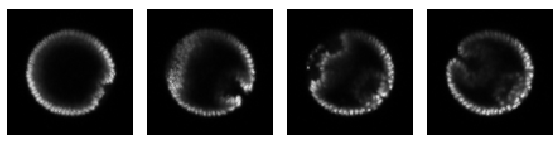
\includegraphics[width=\linewidth]{figures/live}}
\begin{figure}[here]
\livegraphic
\caption{Sample snapshots from a single live movie taken at 5, 10, 15, and 20 minutes. Note that the embryo stays in the same orientation.}
\label{fig:live}
\end{figure}
\newlength{\liveheight}
\settoheight{\liveheight}{\livegraphic}

\begin{figure}[here]
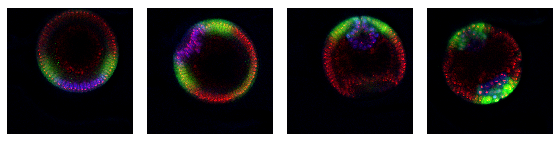
\includegraphics[width=\linewidth]{figures/fixed}
\caption{Sample fixed snapshots. Red is nuclei, while blue and green represent particular proteins. The times and true orientation are not known \textit{a priori}, and the images may be translated or dilated.}
\label{fig:fixed}
\end{figure}

\subsection{Challenges in data preprocessing}

Each live image consists of $100$ by $100$ pixels; fixed snapshots are more but are subsampled. The live movies have just one channel value at each pixel, while the fixed snapshots have three. Each image can thus be viewed as a vector of length $100,000$ (or $300,000$ for fixed snapshots), and a simple first choice of metric is the Euclidean distance between two such vectors. Unfortunately, some significant work needs to be done to make that Euclidean distance informative. The imaging process can produce various image artifacts that are not relevent to the developmental dynamics, especially for the fixed snapshots which are all different embryo. Images need to be centered in the field of view and resized to occupy a consistent portion of the frame. Contrast limited adaptive histogram equalization (CLAHE) is used to normalize the images. We recently found that boosting the contrast significantly improves the performance, probably because whether or not a pixel is occupied is more important than the specific brightness level. Finally, we blur the images using a Gaussian filter to remove small scale structure that distorts the comparison. Variability between embryo means that features will not be in the exact same place; blurring allows such features to be more properly compared.

\begin{figure}[here]
\centering
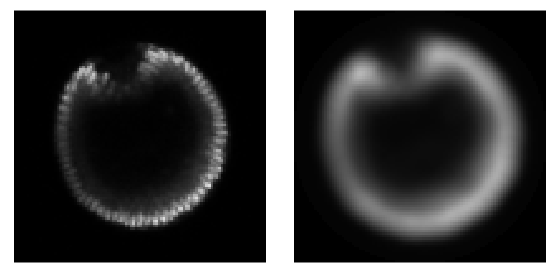
\includegraphics[height=\liveheight]{figures/preprocess} \par
\caption{Example raw image and preprocessed image.}
\label{fig:pp}
\end{figure}

\subsection{Synchronization of rotations and movie times}

While the embryos in the live movies stay at the same orientation throughout development, the embryos in the fixed snapshots can be in any arbitrary orientation within the plane. While manual registration is possible, it is extremely tedious. The eigenvector alignment method is capable of registering the fixed snapshots with respect to each other in just seconds of computational time. As previously discussed, the final orientation is arbitrary, so there is a final step of rotating the snapshots to align with the live movies in order to do any comparison. The eigenvector alignment method also provides a framework for aligning the different live movies and the snapshots with respect to each other, but with only 7 live movies and 1 data set of snapshots, the gains over manual registration are minimal. \vspace{1mm}

Another synchronization of interest is that of movie times.  When diffusion maps is run on multiple live movies simultaneously, we find that within each live movie there is a good monotonic relationship between time and the first diffusion maps coordinate. However, these different functional relationships are offset from each other. We believe that while some of this error is due to noise and embryo variability, issues with experimental design could be causing some of the discrepancy. For example, lack of precision in the fertilization time could mean that the times for one embryo are shifted in relation to another. Differences in ambient temperature or other environmental factors could cause one embryo to develop at a faster rate. We are interesting in finding factors by which to scale and shift the movie times so that they optimally align with each other. If we consider operations of the form
\[
t_j = a_{ij}*t_i+b_{ij}
\]
(i.e., how to scale and shift the times in movie $i$ to align with movie $j$), then the eigenvector alignment method can be used by considering the matrix operator
\[
g_{ij}=
\begin{bmatrix}
1 && 0\\
a_{ij} && b_{ij}
\end{bmatrix}
\]
The pairwise $a_{ij}$ and $b_{ij}$ can by quickly found by minimizing the least squares error between the two relationships for time as a function of the first diffusion maps coordinate. We then form the block matrix G, and the top two eigenvectors can be used to form a block eigenvector which contains the scales and shifts from the globally optimal solution. Again, there are degrees of freedom in the scale and in the shift, so we apply a final scale and shift such that the mean shift that we apply to the data is 0 and the mean log scale we apply is also 0. This is in an effort to modify the data as little as possible, and also to make the algorithm deterministic.

\subsection{Data fusion to construct a representative trajectory}

Our data fusion methodology is based on the assumption that the underlying process of embryonic development is primarily one-dimensional and that the primary dimension is monotonic with time. Different methods of observation (i.e., different imaging techniques) embed this 1D process in a higher-dimensional space. Imaging noise and inter-embryo variability represent high-dimensional noise around this one-dimensional manifold. \vspace{1mm}

The initial attempt at data fusion used the additional assumption that the two data sets (live movies and fixed snapshots) had common information: the channel representing nuclei locations. At this point several algorithms are possible; we considered the following:

\begin{enumerate}
\item Run diffusion maps on common information from the (preprocessed) live movies and fixed snapshots as one data set.
\item Based on the data, develop functional relationships between color values at each pixel and the diffusion maps coordinate.
\item ``Color" the live movies based on these functional relationships.
\item Apply some smoothing to the colored live movies to create a smooth, representative trajectory.
\end{enumerate}

The results from this algorithm unfortunately failed multiple sanity checks. The functional relationships showed rough trends but were unreasonably noisy. The ordering of the fixed snapshots in diffusion maps space was poorly correlated with the ordering obtained by an expert. The fixed snapshots spanned a significantly wider range in diffusion maps space than the live movies did. \vspace{1mm}

While the general noisiness of the system contributes to these problem, another significant problem is comes from difference in imaging techniques. Visual inspection shows clear differences between the snapshots and the live movies, most notably in signal strength in the yolk of the embryo. This is believed to be related to the fact that different nuclei staining methods were used. Because of these issues, we violate the assumption that the two data sets have common information; instead they represent different observation functions of the common information. \vspace{1mm}

One approach to this problem is more manual preprocessing of the fixed snapshots. If they can be adjusted so that the (hidden) observation functions are the same, the algorithm should have more success. We have experimented with removing the signal from the yolk, and the results show significant improvement but are still unsatisfactory. We are still investigating alternative preprocessing methods. \vspace{1mm}

Another approach involves transforming the diffusion maps coordinates of the snapshots to better align with the coordinates of the movies. The challenge is to do so in a robust way that maintains the intra-data-set information while aligning the seperate data sets. We may include more diffusion maps coordinates (i.e., a higher dimensional representation), and consider transoformations that translate and twist but do not stretch. Both approaches are in the stage of manual experimentation; we hope to automate as much as possible when a viable approach is found. \vspace{1mm}

\section{Systems of Interest for Future Work}

This section is focused on systems where we hope to use diffusion maps to enable calculations in the EF framework.

\subsection{Molecular simulation}

The utility of molecular simulation is often constrained by computational limitations. Great strides have been made to circumvent these restrictions through techniques like parallel tempering and umbrella sampling, but researchers are often still limited to very short times and oversimplified molecular models. We hope to improve the speed of these simulations with more robust and systematic model reduction. \vspace{1mm}

An area of molecular simulation that has shown promise for our techniques is protein dynamics and folding. Alanine dipeptide (Ala2) is a common reference molecule for testing of new techniques. It has been well studied experimentally and computationally \cite{Wang2014}, and various studies have shown that its dynamics can be well described using a few coarse variables. In 2003, Hummer et. al. implemented several methods of equation-free analysis based on one of the dihedral angles as the coarse variable \cite{Hummer2003}; in 2009, Frewen et. al. used similar techniques to explore the potential energy landscape using two of the dihedral angles \cite{Frewen2009}. Other work has shown that diffusion maps can characterize the dynamics and find good coarse variables. Nedialkov et. al. recently used diffusion maps to parametrize the more complicated alanine pentapeptide, and used the results in clustering algorithm to develop a Markov model \cite{Nedialkova2014}. Ferguson et. al. showed that application of diffusion maps can recover the dihedral angles as coarse variables, and proposed a method to iteratively incorporate diffusion maps variables into successive rounds of umbrella sampling \cite{Ferguson2011}. \vspace{1mm}

We would like to combine the diffusion maps approach with the EF framework and show that diffusion maps can provide good coarse variables for EF methods to use. One issue noted in the Ferguson work is that their is no systematic method for determining physical variables for umbrella samplling that the diffusion maps variables parameterize. However, in the EF framework, the functional relationship between diffusion maps coordinates and physical parameters only needs to be known on the scale of the coarse time step, not globally. This should be feasible using the lifting and restriction operators described in section \ref{DMLR}.

\subsection{Reaction networks}

Diffusion maps has been shown to parameterize reaction networks represented by systems of ODEs \cite{Chiavazzo2014}. This is one of the few areas where diffusion maps has been used to improve calculations rather than clarity; Chivazzo et. al. used their work to develop a reduced model using lifting and restriction operators. However, they still used the framework of data collection followed by model formulation, and they note that improvements could be made by using the diffusion maps coordinates to extend the manifold. The main computational cost of constructing the model involves sufficiently sampling the manifold; this could potentially be reduced by using the diffusion maps coordinates to predict which new evaluations will give more information about parts of the manifold that haven't yet been explored. \vspace{1mm}

Diffusion maps can also be applied to reaction networks described by stochastic simulation rather than continuous ODEs \cite{Dsilva2013}.The Gillespie stochastic simulation algorithm (SSA) is an efficient method for simulating reactions in systems with relatively small numbers of molecules, where the stochastic nature of reaction kinetics is not averaged out \cite{Gillespie1977}. Based on the number of molecules in the system and the rate constants of possible reactions, SSA calculates probability distributions for each reaction occuring in a given time window. Based on these distributions, a reaction and time to reaction are selected randomly; the SSA procedes forward by repeatedly selecting the next reaction to take place. The stochastic nature of the simulation suggests the use of the Mahalonobis distance in diffusion maps to factor out the noise and discover the slow manifold that systems drifts on.

\section{Conclusions}

The equation-free framework has been demonstrated to improve computational tractability in detailed systems that can be effectively parameterized by a low-dimensional, coarse description. This methodology depends primarily on discovering the coarse variables as well as efficient lifting and restriction operators to move between coarse and fine variables. A major stumbling block is the ability to determine these coarse variables systematically without \textit{a priori} information about the dynamics. \vspace{1mm}

Diffusion maps is a manifold learning method that has been shown to effectively discover low dimensional descriptions of complex data in systems ranging from developmental biology to molecular dynamics. To this point, it has been used primarily to improve clarity of the dynamics. Only very recently has work been done using diffusion maps to improve the efficency of calculations, but methods to this point have relied either on fully collecting the data set before hand, or on manual correlation of diffusion maps coordinates with globally applicable physical variables. \vspace{1mm}

The combinations of these approaches has applications in all fields of computational modeling. We hope to demonstrate the viability of diffusion maps to enable use of equation-free modeling in molecular dynamics and reaction kinetics.

\bibliographystyle{abbrv}
\bibliography{../first-prop}
\end{document}